
\section{OpenNebula}

OpenNebula is a useful opensource that enables seamless management and
control of different cloud systems.  The tools can be used for a cloud
implementations to virtualize data centers and also to obtain solution
for cloud infrastructure.  Opennebula can be adopted on top of an
existing cloud setup.  OpenNebula project started on 2005 and
currently the product is available as an open-source under Apache
license.
``The toolkit includes features for integration, management,
scalability, security and accounting.  It also claims standardization,
interoperability and portability, providing cloud users and
administrators with a choice of several cloud interfaces (Amazon EC2
Query, OGF Open Cloud Computing Interface and vCloud) and hypervisors
(Xen, KVM and VMware), and can accommodate multiple hardware and
software combinations in a data
center''~\cite{hid-sp18-417-opennebula-wiki}.

\begin{figure}[htb]
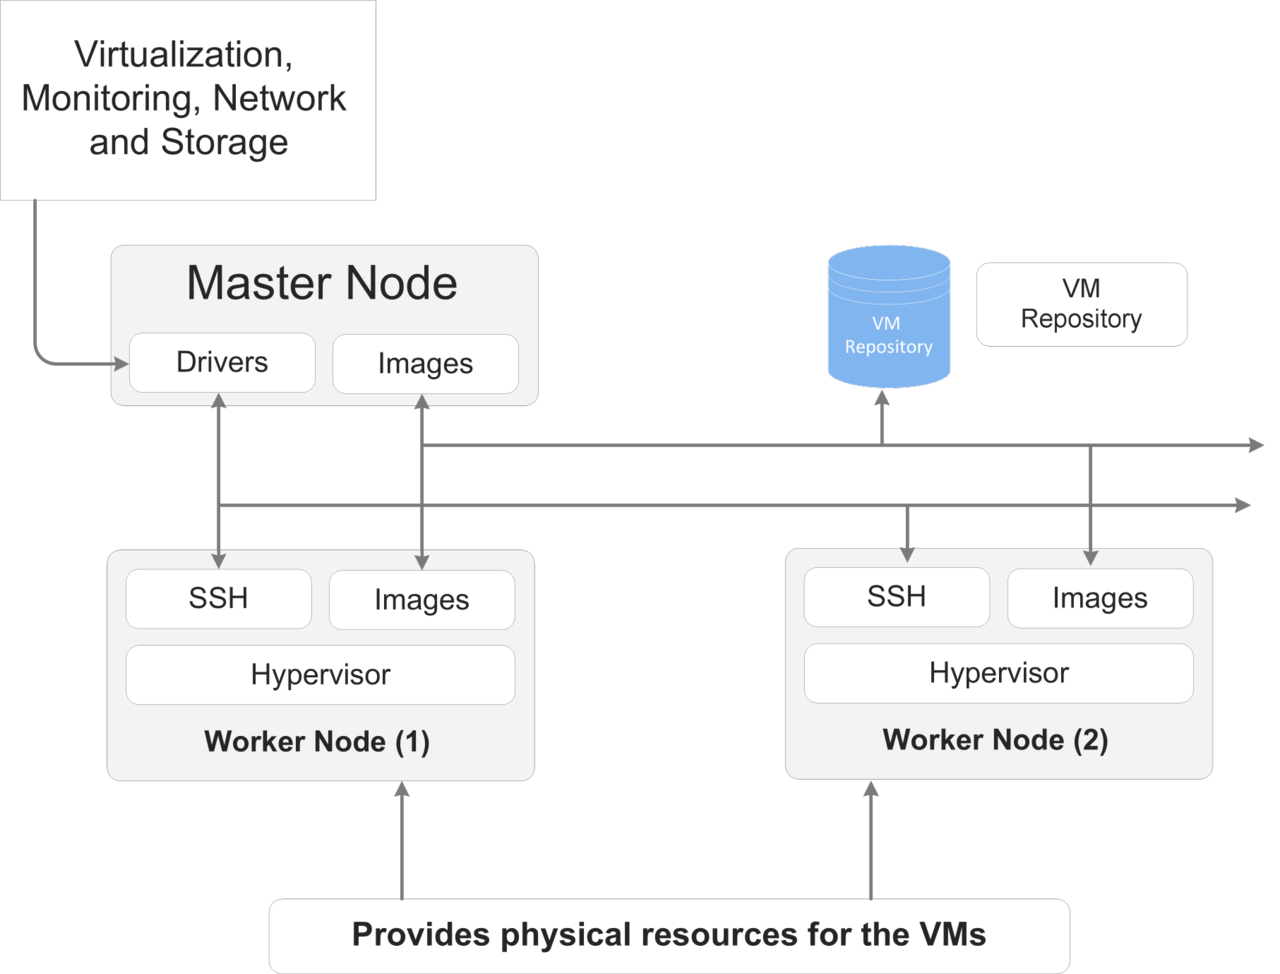
\includegraphics[width=\textwidth]{images/hid-sp18-417-opennebula.png}
\caption{OpenNebula Deployment Model~\cite{hid-sp18-417-opennebula-deployment}} 
\label{F:opennebula}
\end{figure}


The OpenNebula deployment needs (1) A client node (2) A hypervisor (3)
A data storage system (4) Physical network.  The deployment model is
depicted in~\ref{F:opennebula}.  Due to its long steady growth, the
tool is being used by customers in various industries ranging from
telecom to education.  The wide range of customer base is helpful in
providing a solid support system to the new and existing users as well
as continuous feedback becomes vital in the research and growth of the
project.
